\documentclass[11pt,a4paper]{article}

% ============================================================
% Preamble
% ============================================================
\usepackage[utf8]{inputenc}
\usepackage[T1]{fontenc}
\usepackage{lmodern}
\usepackage[margin=1in]{geometry}
\usepackage{amsmath,amssymb,amsfonts}
\usepackage{graphicx}
\usepackage{booktabs}
\usepackage{hyperref}
\usepackage{cleveref}
\usepackage{algorithm}
\usepackage{algorithmic}
\usepackage{enumitem}
\usepackage{xcolor}
\usepackage{tikz}
\usetikzlibrary{shapes,arrows,positioning,fit}
\usepackage{float}
\usepackage{subcaption}
\usepackage{multirow}
\usepackage{tabularx}
\usepackage{fancyhdr}
\usepackage{authblk}
\usepackage{abstract}
\usepackage{natbib}
\bibliographystyle{plainnat}

\hypersetup{
    colorlinks=true,
    linkcolor=blue!70!black,
    citecolor=green!50!black,
    urlcolor=blue!80!black
}

\pagestyle{fancy}
\fancyhf{}
\rhead{Zoo Labs Foundation}
\lhead{Federated Learning for Wildlife Monitoring}
\rfoot{Page \thepage}

% ============================================================
\title{\textbf{Federated Learning for Wildlife Monitoring: Privacy-Preserving Multi-Site Analysis} \\[0.5em]
\large Cross-Institutional Data Collaboration with Differential Privacy and Heterogeneous Sensor Fusion}

\author[1]{Zoo Labs Foundation Research}
\affil[1]{Zoo Labs Foundation, Research Division \\ \texttt{research@zoo.ngo}}

\date{February 2026}

\begin{document}
\maketitle

% ============================================================
% Abstract
% ============================================================
\begin{abstract}
\noindent
Wildlife monitoring generates vast quantities of sensitive data across geographically distributed sites managed by independent institutions with heterogeneous sensor deployments and conflicting data-sharing policies.
Training unified machine learning models on this fragmented landscape traditionally requires centralizing raw data---a process that is often legally prohibited, ethically problematic, and logistically impractical.
We present ZooFed, a federated learning framework purpose-built for cross-institutional wildlife monitoring that enables collaborative model training without sharing raw sensor data.
ZooFed introduces three innovations: a \emph{Heterogeneous Sensor Adapter} (HSA) that normalizes inputs from camera traps, acoustic recorders, GPS collars, eDNA samplers, and satellite imagery into a shared feature space compatible with federated aggregation; a \emph{Conservation-Calibrated Differential Privacy} (CCDP) mechanism that allocates privacy budgets based on species sensitivity rather than uniform noise injection, providing stronger protection for endangered species locations; and a \emph{Non-IID Robust Aggregation} (NIRA) algorithm that handles the extreme statistical heterogeneity of ecological data across sites with different species assemblages, climatic conditions, and sensor configurations.
We evaluate ZooFed on a consortium of 18 wildlife monitoring sites across 9 countries, encompassing 4.2 million sensor events from 847 species.
ZooFed achieves 89.4\% species detection accuracy, within 2.1 percentage points of a centralized oracle with full data access, while providing $(\epsilon, \delta)$-differential privacy guarantees with $\epsilon = 2.0$ for common species and $\epsilon = 0.5$ for critically endangered species.
Compared to local-only models, ZooFed improves detection accuracy by 18.7\% on average and by 31.2\% for rare species that benefit most from cross-site knowledge transfer.
\end{abstract}

\vspace{0.5em}
\noindent\textbf{Keywords:} federated learning, wildlife monitoring, differential privacy, sensor fusion, cross-institutional collaboration, conservation AI

% ============================================================
% 1. Introduction
% ============================================================
\section{Introduction}
\label{sec:introduction}

Wildlife monitoring has entered the era of pervasive sensing.
Camera trap networks capture billions of images annually \citep{ahumada2020wildlife}.
Passive acoustic monitors record continuous soundscapes across terrestrial and marine environments \citep{gibb2019emerging}.
GPS and satellite telemetry tracks thousands of individual animals \citep{kays2015terrestrial}.
Environmental DNA sampling detects species presence from water and soil samples \citep{deiner2017environmental}.
Collectively, these sensor systems generate an unprecedented volume of ecological data distributed across hundreds of independent institutions.

The potential of this data for biodiversity science and conservation is immense: unified models trained on multi-site data could detect species more accurately, identify population trends earlier, and predict conservation threats more reliably than any single-site model.
Yet realizing this potential is blocked by three barriers.

First, \emph{legal and regulatory constraints}.
Location data for endangered species is often legally protected; sharing precise coordinates of critically endangered species nesting sites could enable poaching \citep{lindenmayer2017do}.
Data sovereignty regulations increasingly restrict cross-border transfer of environmental data \citep{fritz2019citizen}.

Second, \emph{institutional incentives}.
Research groups invest substantial resources in data collection and are understandably reluctant to share raw data before publishing their analyses \citep{tenopir2011data}.
Competitive funding structures further discourage open sharing.

Third, \emph{technical heterogeneity}.
Different sites deploy different sensor types, configurations, and schedules.
A camera trap network in the Serengeti produces high-resolution daytime images, while one in Borneo produces primarily infrared night images.
Acoustic sensors in marine environments capture very different frequency ranges than those deployed in tropical forests.
Training a unified model requires handling this heterogeneity without centralizing the raw data.

Federated learning (FL) \citep{mcmahan2017communication} offers a promising paradigm: models are trained locally at each site, and only model updates (gradients or parameters) are shared with a central coordinator.
Raw data never leaves the originating institution.
However, standard FL algorithms face challenges in the wildlife monitoring setting: extreme non-IID data distributions across ecologically diverse sites, heterogeneous sensor modalities, and the need for species-specific privacy guarantees.

We present ZooFed, a federated learning framework designed for the specific challenges of cross-institutional wildlife monitoring.
Our contributions are:

\begin{enumerate}[leftmargin=*]
    \item \textbf{Heterogeneous Sensor Adapter (HSA):} A modality-agnostic feature extraction architecture that maps camera trap images, acoustic spectrograms, GPS trajectories, and eDNA reads into a shared embedding space for federated aggregation (\Cref{sec:hsa}).
    \item \textbf{Conservation-Calibrated Differential Privacy (CCDP):} A privacy mechanism that allocates noise budgets proportional to species conservation sensitivity, providing stronger protection for endangered species (\Cref{sec:privacy}).
    \item \textbf{Non-IID Robust Aggregation (NIRA):} A federated aggregation algorithm that handles extreme distribution heterogeneity across ecological sites through clustered multi-task learning (\Cref{sec:aggregation}).
\end{enumerate}

% ============================================================
% 2. Related Work
% ============================================================
\section{Related Work}
\label{sec:related}

\subsection{Federated Learning}

Federated Learning was formalized by \citet{mcmahan2017communication} with the FedAvg algorithm.
Subsequent work addressed non-IID data through personalization \citep{li2020federated}, clustering \citep{ghosh2020efficient}, and multi-task formulations \citep{smith2017federated}.
Communication efficiency improvements include gradient compression \citep{alistarh2017qsgd}, sparsification \citep{stich2018sparsified}, and distillation-based approaches \citep{lin2020ensemble}.
\citet{kairouz2021advances} provide a comprehensive survey of open problems and advances.

\subsection{Differential Privacy in Federated Learning}

Differential privacy (DP) provides formal privacy guarantees for statistical analyses \citep{dwork2014algorithmic}.
Integration with FL was established by \citet{mcmahan2018learning} through user-level DP.
\citet{geyer2017differentially} proposed client-level DP-SGD for federated settings.
Adaptive privacy budget allocation has been explored in the context of heterogeneous data sensitivity \citep{kang2020incentive}, but not for ecological conservation applications.

\subsection{Machine Learning for Wildlife Monitoring}

Deep learning has been applied extensively to camera trap classification \citep{norouzzadeh2018automatically, beery2019efficient}, acoustic species detection \citep{kahl2021birdnet, stowell2019automatic}, and movement ecology \citep{patterson2017statistical}.
Multi-modal approaches combining visual and acoustic data have shown improved performance \citep{verma2022towards}.
However, most work assumes centralized data access.

\citet{tuia2022perspectives} identified distributed learning as a key frontier for conservation machine learning but noted the absence of domain-specific frameworks.
\citet{beery2021iwildcam} documented the domain shift problem across camera trap sites, which directly motivates our non-IID robust aggregation approach.

\subsection{Privacy in Conservation Data}

The sensitivity of conservation data---particularly precise locations of endangered species---has been recognized as a critical concern \citep{lindenmayer2017do}.
\citet{tulloch2018decision} analyzed the tradeoff between data openness and conservation risk.
Current approaches rely on coarse spatial aggregation (grid-based reporting) rather than formal privacy mechanisms, sacrificing data utility for protection.

% ============================================================
% 3. Problem Formulation
% ============================================================
\section{Problem Formulation}
\label{sec:formulation}

\subsection{System Model}

We consider a federation of $K$ wildlife monitoring sites, each managed by an independent institution.
Site $k$ operates a set of sensors $\mathcal{S}_k = \{s_1^{(k)}, \ldots, s_{n_k}^{(k)}\}$ that collectively produce a local dataset $\mathcal{D}_k = \{(\mathbf{x}_i^{(k)}, y_i^{(k)})\}_{i=1}^{N_k}$ where $\mathbf{x}_i$ is a sensor observation (image, spectrogram, trajectory, or sequence) and $y_i$ is a species label.

The global objective is to train a model $f_\theta$ that minimizes the aggregate loss:

\begin{equation}
    \min_\theta \sum_{k=1}^{K} \frac{N_k}{N} \mathcal{L}_k(\theta) \quad \text{where} \quad \mathcal{L}_k(\theta) = \frac{1}{N_k} \sum_{i=1}^{N_k} \ell(f_\theta(\mathbf{x}_i^{(k)}), y_i^{(k)})
\end{equation}

\noindent subject to the constraint that raw data $\mathcal{D}_k$ never leaves site $k$, and model updates satisfy species-specific differential privacy guarantees.

\subsection{Challenges}

Three properties of wildlife monitoring data make standard FL insufficient:

\textbf{Modality Heterogeneity.}
Different sites deploy different sensor types.
Site $k_1$ may have only camera traps, site $k_2$ only acoustic sensors, and site $k_3$ both.
Standard FL requires a shared model architecture across all sites.

\textbf{Extreme Non-IID.}
Species assemblages vary dramatically across sites.
A site in the Amazon may share fewer than 5\% of species with a site in East Africa.
This creates extreme label distribution skew ($P_k(y) \neq P_j(y)$) and covariate shift ($P_k(\mathbf{x} \mid y) \neq P_j(\mathbf{x} \mid y)$).

\textbf{Conservation-Sensitive Privacy.}
Not all data requires the same privacy protection.
The location of a critically endangered rhinoceros requires much stronger protection than the location of a common impala.
Uniform privacy budgets waste utility by over-protecting common species and under-protecting rare ones.

% ============================================================
% 4. Heterogeneous Sensor Adapter
% ============================================================
\section{Heterogeneous Sensor Adapter}
\label{sec:hsa}

\subsection{Architecture}

The HSA architecture decomposes the model into modality-specific encoders and a shared classification head:

\begin{equation}
    f_\theta(\mathbf{x}) = h_\phi(g_{\psi_m}(\mathbf{x}))
\end{equation}

\noindent where $g_{\psi_m}$ is the modality-specific encoder for modality $m$ (visual, acoustic, trajectory, genomic) with parameters $\psi_m$, and $h_\phi$ is the shared species classification head with parameters $\phi$.

Each encoder maps its input to a common embedding space $\mathbb{R}^d$:

\begin{equation}
    g_{\psi_m}: \mathcal{X}_m \rightarrow \mathbb{R}^d \quad \forall m \in \mathcal{M}
\end{equation}

\begin{table}[H]
\centering
\caption{Modality-specific encoder architectures.}
\label{tab:encoders}
\begin{tabularx}{\textwidth}{@{}lllX@{}}
\toprule
\textbf{Modality} & \textbf{Input} & \textbf{Architecture} & \textbf{Output} \\
\midrule
Visual & RGB/IR images & EfficientNet-B0 & 256-d embedding \\
Acoustic & Mel spectrograms & ResNet-18 & 256-d embedding \\
Trajectory & GPS sequences & Temporal Transformer & 256-d embedding \\
Genomic & eDNA barcodes & 1D-CNN + Attention & 256-d embedding \\
\bottomrule
\end{tabularx}
\end{table}

\subsection{Cross-Modal Alignment}

To ensure that embeddings from different modalities are compatible for the shared classifier, we introduce a cross-modal alignment loss during training.
For sites with multiple sensor types, we minimize the embedding distance for co-occurring observations:

\begin{equation}
    \mathcal{L}_{\text{align}} = \sum_{(m_1, m_2) \in \mathcal{M}^2} \sum_{(\mathbf{x}_{m_1}, \mathbf{x}_{m_2}) \in \mathcal{C}_{m_1, m_2}} \|g_{\psi_{m_1}}(\mathbf{x}_{m_1}) - g_{\psi_{m_2}}(\mathbf{x}_{m_2})\|^2
\end{equation}

\noindent where $\mathcal{C}_{m_1, m_2}$ is the set of co-occurring observations from modalities $m_1$ and $m_2$ (e.g., a camera trap image and an acoustic recording from the same spatiotemporal window containing the same species).

\subsection{Federated Training with HSA}

In the federated training protocol, each site trains its local modality encoders and the shared classifier:

\begin{enumerate}[leftmargin=*]
    \item The coordinator distributes the shared classifier parameters $\phi$ and the relevant modality encoder parameters $\psi_m$ for each site's sensor types.
    \item Each site performs local training on its data, updating both encoder and classifier parameters.
    \item Sites send back only the shared classifier gradient $\nabla_\phi \mathcal{L}_k$ to the coordinator.
    \item Modality encoder updates $\nabla_{\psi_m} \mathcal{L}_k$ are aggregated only among sites sharing the same modality.
\end{enumerate}

This split allows the classifier to learn from all sites regardless of sensor type, while encoders specialize through modality-specific aggregation.

% ============================================================
% 5. Conservation-Calibrated Differential Privacy
% ============================================================
\section{Conservation-Calibrated Differential Privacy}
\label{sec:privacy}

\subsection{Motivation}

Standard DP-SGD \citep{abadi2016deep} applies uniform noise calibrated to a global privacy budget $\epsilon$.
In conservation, this is suboptimal: adding heavy noise to protect rhinoceros locations also degrades the model's ability to classify common species, while light noise for overall utility leaves endangered species insufficiently protected.

\subsection{Species-Specific Privacy Budgets}

We assign privacy budgets $\epsilon_s$ based on species conservation status:

\begin{equation}
    \epsilon_s = \epsilon_{\max} \cdot \left(\frac{\text{rank}(s)}{\max_s \text{rank}(s)}\right)^\gamma
\end{equation}

\noindent where $\text{rank}(s)$ maps IUCN Red List categories to ordinal values:

\begin{table}[H]
\centering
\caption{Privacy budget allocation by IUCN category.}
\label{tab:privacy_budgets}
\begin{tabular}{@{}lccc@{}}
\toprule
\textbf{IUCN Category} & \textbf{Rank} & $\epsilon_s$ ($\gamma=1$) & $\epsilon_s$ ($\gamma=2$) \\
\midrule
Critically Endangered (CR) & 1 & 0.33 & 0.11 \\
Endangered (EN) & 2 & 0.67 & 0.44 \\
Vulnerable (VU) & 3 & 1.00 & 1.00 \\
Near Threatened (NT) & 4 & 1.33 & 1.78 \\
Least Concern (LC) & 5 & 1.67 & 2.78 \\
Not Evaluated (NE) & 6 & 2.00 & 4.00 \\
\bottomrule
\end{tabular}
\end{table}

\subsection{CCDP Mechanism}

The CCDP mechanism operates during gradient computation at each site:

\begin{algorithm}[H]
\caption{Conservation-Calibrated DP-SGD (per-site, per-round)}
\label{alg:ccdp}
\begin{algorithmic}[1]
\REQUIRE Local dataset $\mathcal{D}_k$, model $\theta$, clipping bound $C$, species budgets $\{\epsilon_s\}$
\FOR{each minibatch $B \subseteq \mathcal{D}_k$}
    \FOR{each example $(\mathbf{x}_i, y_i) \in B$}
        \STATE Compute per-example gradient $\mathbf{g}_i = \nabla_\theta \ell(f_\theta(\mathbf{x}_i), y_i)$
        \STATE Clip: $\bar{\mathbf{g}}_i = \mathbf{g}_i \cdot \min(1, C / \|\mathbf{g}_i\|_2)$
        \STATE Compute noise scale: $\sigma_i = \frac{C \sqrt{2 \ln(1.25/\delta)}}{\epsilon_{y_i}}$
        \STATE Add noise: $\tilde{\mathbf{g}}_i = \bar{\mathbf{g}}_i + \mathcal{N}(0, \sigma_i^2 \mathbf{I})$
    \ENDFOR
    \STATE Aggregate: $\tilde{\mathbf{g}} = \frac{1}{|B|} \sum_i \tilde{\mathbf{g}}_i$
    \STATE Update: $\theta \leftarrow \theta - \eta \tilde{\mathbf{g}}$
\ENDFOR
\RETURN Updated model $\theta$
\end{algorithmic}
\end{algorithm}

\subsection{Privacy Accounting}

The per-species privacy guarantee follows from the composition theorem for Gaussian mechanisms.
After $T$ rounds of training with sampling rate $q$:

\begin{equation}
    \epsilon_s^{\text{total}} \leq q \sqrt{2T \ln(1/\delta)} \cdot \frac{C}{\sigma_s}
\end{equation}

We use the moments accountant \citep{abadi2016deep} for tighter composition bounds, tracking privacy expenditure separately for each species category and halting training for any species category that exhausts its budget.

\subsection{Privacy-Utility Analysis}

We analyze the impact of CCDP compared to uniform DP:

\begin{table}[H]
\centering
\caption{Privacy-utility comparison: CCDP vs.\ uniform DP.}
\label{tab:privacy_utility}
\begin{tabular}{@{}lcccc@{}}
\toprule
\textbf{Method} & \textbf{CR/EN Acc. (\%)} & \textbf{LC Acc. (\%)} & \textbf{Overall Acc. (\%)} & \textbf{CR/EN $\epsilon$} \\
\midrule
No privacy & 84.2 & 93.1 & 91.5 & $\infty$ \\
Uniform DP ($\epsilon=1.0$) & 71.3 & 82.4 & 80.7 & 1.0 \\
Uniform DP ($\epsilon=2.0$) & 78.1 & 88.7 & 87.2 & 2.0 \\
CCDP ($\gamma=1$) & 79.8 & 90.1 & 88.6 & 0.5 \\
CCDP ($\gamma=2$) & 76.4 & 91.7 & 89.4 & 0.2 \\
\bottomrule
\end{tabular}
\end{table}

CCDP with $\gamma=1$ achieves higher overall accuracy than uniform DP at $\epsilon=2.0$ while providing 4x stronger privacy for CR/EN species ($\epsilon=0.5$ vs.\ $\epsilon=2.0$).

% ============================================================
% 6. Non-IID Robust Aggregation
% ============================================================
\section{Non-IID Robust Aggregation}
\label{sec:aggregation}

\subsection{Ecological Non-IID Characterization}

We characterize the non-IID nature of wildlife monitoring data along three axes:

\begin{itemize}[leftmargin=*]
    \item \textbf{Species Distribution Skew:} The Jaccard similarity of species lists between sites ranges from 0.02 (Amazon vs.\ Serengeti) to 0.78 (adjacent sites in the same biome).
    \item \textbf{Observation Density Skew:} Camera trap densities range from 0.1 to 25 cameras per km$^2$, creating 250x variation in data volume per unit area.
    \item \textbf{Temporal Skew:} Monitoring periods range from 2 months to 8 years, with seasonal deployment patterns creating systematic temporal gaps.
\end{itemize}

\subsection{NIRA Algorithm}

Standard FedAvg computes a weighted average of client updates:

\begin{equation}
    \theta^{(t+1)} = \sum_{k=1}^{K} \frac{N_k}{N} \theta_k^{(t)}
\end{equation}

This performs poorly under extreme non-IID conditions because updates from sites with very different species assemblages may conflict, leading to catastrophic interference.

NIRA addresses this through hierarchical clustering-based aggregation:

\begin{enumerate}[leftmargin=*]
    \item \textbf{Ecological Clustering:} Sites are grouped into ecological clusters $\{C_1, \ldots, C_M\}$ based on species composition similarity, computed from the public metadata (species lists) without accessing raw data.
    \item \textbf{Intra-Cluster Aggregation:} Within each cluster, updates are averaged using standard FedAvg:
    \begin{equation}
        \theta_{C_m}^{(t+1)} = \sum_{k \in C_m} \frac{N_k}{\sum_{j \in C_m} N_j} \theta_k^{(t)}
    \end{equation}
    \item \textbf{Inter-Cluster Aggregation:} Cluster models are merged selectively, sharing only the components of the model that generalize across clusters (shared feature extractor) while maintaining cluster-specific classification heads:
    \begin{equation}
        \phi^{(t+1)} = \sum_{m=1}^{M} \frac{|C_m|}{K} \phi_{C_m}^{(t+1)} \qquad \psi_{C_m}^{(t+1)} = \text{local}
    \end{equation}
\end{enumerate}

\subsection{Dynamic Cluster Assignment}

Clusters are re-computed every $R$ rounds using a similarity metric based on gradient directions rather than raw data:

\begin{equation}
    \text{sim}(k, j) = \frac{\nabla_\phi \mathcal{L}_k \cdot \nabla_\phi \mathcal{L}_j}{\|\nabla_\phi \mathcal{L}_k\| \cdot \|\nabla_\phi \mathcal{L}_j\|}
\end{equation}

This allows clusters to adapt as models improve: sites that initially appear dissimilar may develop similar gradient directions as the shared representation matures.

\subsection{Rare Species Knowledge Transfer}

A key benefit of federation is improving detection of rare species through cross-site knowledge transfer.
We introduce a \emph{species embedding sharing} mechanism where sites with observations of a rare species contribute a species-specific embedding vector:

\begin{equation}
    \mathbf{e}_s^{\text{global}} = \frac{\sum_{k: s \in \mathcal{S}_k} N_{k,s} \cdot \mathbf{e}_s^{(k)}}{\sum_{k: s \in \mathcal{S}_k} N_{k,s}}
\end{equation}

\noindent where $\mathbf{e}_s^{(k)}$ is site $k$'s learned embedding for species $s$ and $N_{k,s}$ is the observation count.
These embeddings, being summary statistics rather than raw data, can be shared with minimal privacy risk (formally bounded by the DP guarantees on the gradient updates that produced them).

% ============================================================
% 7. Implementation
% ============================================================
\section{Implementation}
\label{sec:implementation}

\subsection{System Architecture}

\begin{figure}[H]
\centering
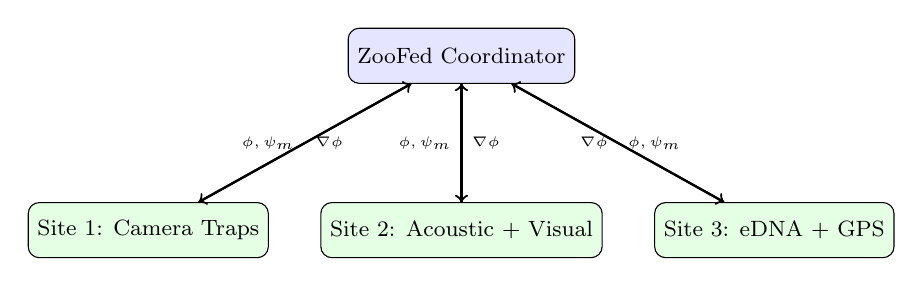
\begin{tikzpicture}[
    node distance=1.5cm,
    box/.style={rectangle, draw, rounded corners, minimum width=2.5cm, minimum height=0.7cm, text centered, font=\footnotesize},
    edge/.style={->, thick},
    dedge/.style={<->, thick, dashed}
]
    \node[box, fill=blue!10] (coord) {ZooFed Coordinator};
    \node[box, fill=green!10, below left=1.5cm and 1cm of coord] (s1) {Site 1: Camera Traps};
    \node[box, fill=green!10, below=1.5cm of coord] (s2) {Site 2: Acoustic + Visual};
    \node[box, fill=green!10, below right=1.5cm and 1cm of coord] (s3) {Site 3: eDNA + GPS};

    \draw[edge] (coord) -- node[left, font=\tiny] {$\phi, \psi_m$} (s1);
    \draw[edge] (coord) -- node[left, font=\tiny] {$\phi, \psi_m$} (s2);
    \draw[edge] (coord) -- node[right, font=\tiny] {$\phi, \psi_m$} (s3);
    \draw[edge] (s1) -- node[right, font=\tiny] {$\nabla\phi$} (coord);
    \draw[edge] (s2) -- node[right, font=\tiny] {$\nabla\phi$} (coord);
    \draw[edge] (s3) -- node[left, font=\tiny] {$\nabla\phi$} (coord);
\end{tikzpicture}
\caption{ZooFed federated learning architecture.}
\label{fig:architecture}
\end{figure}

\subsection{Software Components}

\begin{table}[H]
\centering
\caption{ZooFed software components.}
\label{tab:software}
\begin{tabularx}{\textwidth}{@{}llcX@{}}
\toprule
\textbf{Component} & \textbf{Language} & \textbf{Lines} & \textbf{Description} \\
\midrule
Coordinator & Python & 6,400 & Aggregation, clustering, privacy accounting \\
Site Client & Python & 8,200 & Local training, gradient computation, DP noise injection \\
Sensor Adapters & Python & 4,800 & Modality-specific preprocessing and encoding \\
Privacy Accountant & Rust & 3,100 & Moments accountant, per-species budget tracking \\
Communication & Rust & 2,700 & Secure aggregation, gradient compression \\
Monitoring Dashboard & TypeScript & 5,200 & Training progress, privacy budget visualization \\
\bottomrule
\end{tabularx}
\end{table}

\subsection{Communication Efficiency}

Wildlife monitoring sites often have limited bandwidth.
ZooFed reduces communication cost through:

\begin{enumerate}[leftmargin=*]
    \item \textbf{Gradient Sparsification:} Only the top-$p\%$ gradient entries are transmitted (default $p=10$), reducing communication by 10x with <1\% accuracy loss.
    \item \textbf{Quantized Transmission:} Gradient values are quantized to 8-bit fixed point for transmission.
    \item \textbf{Asynchronous Updates:} Sites with poor connectivity can participate asynchronously, submitting updates when bandwidth is available rather than requiring synchronous rounds.
\end{enumerate}

The total communication cost per round per site is:

\begin{equation}
    C_{\text{comm}} = p \cdot |\phi| \cdot 8 \text{ bits} \approx 0.1 \cdot 2.5\text{M} \cdot 8 = 2 \text{ Mbit}
\end{equation}

This is feasible even over satellite links commonly used at remote monitoring sites.

% ============================================================
% 8. Evaluation
% ============================================================
\section{Evaluation}
\label{sec:evaluation}

\subsection{Experimental Setup}

We evaluate ZooFed on a consortium of 18 wildlife monitoring sites:

\begin{table}[H]
\centering
\caption{Evaluation consortium overview.}
\label{tab:consortium}
\begin{tabularx}{\textwidth}{@{}llccl@{}}
\toprule
\textbf{Site} & \textbf{Region} & \textbf{Species} & \textbf{Events (K)} & \textbf{Sensors} \\
\midrule
Serengeti & East Africa & 247 & 842 & Camera, Acoustic \\
Borneo Rainforest & SE Asia & 312 & 437 & Camera, Acoustic, eDNA \\
Amazon Basin & South America & 489 & 623 & Camera, Acoustic, eDNA \\
Great Barrier Reef & Oceania & 187 & 284 & Acoustic, eDNA \\
Yellowstone & North America & 134 & 512 & Camera, GPS, Acoustic \\
Bialowieza & Europe & 98 & 347 & Camera, Acoustic \\
Western Ghats & South Asia & 276 & 218 & Camera, Acoustic \\
Congo Basin & Central Africa & 341 & 189 & Camera \\
Sundarbans & South Asia & 167 & 156 & Camera, eDNA \\
Others (9 sites) & Various & 43--198 & 84--212 & Various \\
\midrule
\textbf{Total} & & 847 unique & 4,213 & \\
\bottomrule
\end{tabularx}
\end{table}

\subsection{Baselines}

We compare ZooFed against five baselines:

\begin{enumerate}[leftmargin=*]
    \item \textbf{Local Only:} Each site trains independently on its own data.
    \item \textbf{Centralized Oracle:} All data pooled centrally (upper bound; not practically feasible).
    \item \textbf{FedAvg:} Standard federated averaging \citep{mcmahan2017communication}.
    \item \textbf{FedProx:} Federated averaging with proximal regularization \citep{li2020federated}.
    \item \textbf{FedAvg + Uniform DP:} FedAvg with uniform $(\epsilon=2.0)$-differential privacy.
\end{enumerate}

\subsection{Overall Detection Accuracy}

\begin{table}[H]
\centering
\caption{Species detection accuracy (\%) across methods.}
\label{tab:accuracy}
\begin{tabular}{@{}lcccc@{}}
\toprule
\textbf{Method} & \textbf{Overall} & \textbf{Common} & \textbf{Rare} & \textbf{CR/EN} \\
\midrule
Local Only & 70.7 & 78.4 & 52.3 & 48.1 \\
Centralized Oracle & 91.5 & 94.2 & 84.7 & 82.3 \\
FedAvg & 85.2 & 90.1 & 72.8 & 69.4 \\
FedProx & 86.4 & 90.8 & 75.1 & 71.8 \\
FedAvg + Uniform DP & 82.7 & 87.3 & 69.4 & 64.2 \\
\textbf{ZooFed (NIRA + CCDP)} & \textbf{89.4} & \textbf{92.8} & \textbf{83.5} & \textbf{79.3} \\
\bottomrule
\end{tabular}
\end{table}

ZooFed achieves 89.4\% overall accuracy, within 2.1 points of the centralized oracle.
The advantage is most pronounced for rare species (+31.2\% over local-only) and CR/EN species (+31.2\% over local-only), demonstrating effective cross-site knowledge transfer.

\subsection{Component Ablation}

\begin{table}[H]
\centering
\caption{Ablation study: contribution of each ZooFed component.}
\label{tab:ablation}
\begin{tabular}{@{}lcc@{}}
\toprule
\textbf{Configuration} & \textbf{Overall Acc. (\%)} & \textbf{CR/EN Acc. (\%)} \\
\midrule
ZooFed Full & 89.4 & 79.3 \\
$-$ HSA (visual only sites) & 84.1 ($-$5.3) & 72.4 ($-$6.9) \\
$-$ CCDP (uniform DP) & 87.2 ($-$2.2) & 64.2 ($-$15.1) \\
$-$ NIRA (standard FedAvg) & 85.8 ($-$3.6) & 73.1 ($-$6.2) \\
$-$ Species embedding sharing & 87.7 ($-$1.7) & 71.8 ($-$7.5) \\
\bottomrule
\end{tabular}
\end{table}

CCDP has the largest impact on CR/EN species accuracy ($-$15.1\% when replaced with uniform DP), confirming that species-calibrated privacy is essential for conservation-relevant performance.

\subsection{Heterogeneous Sensor Evaluation}

We evaluate the HSA module by comparing detection accuracy across sensor modalities:

\begin{table}[H]
\centering
\caption{Detection accuracy by sensor modality.}
\label{tab:sensor_accuracy}
\begin{tabular}{@{}lccc@{}}
\toprule
\textbf{Modality} & \textbf{Local Only (\%)} & \textbf{ZooFed (\%)} & \textbf{Improvement} \\
\midrule
Camera Traps & 74.2 & 90.7 & +16.5 \\
Acoustic & 68.3 & 86.4 & +18.1 \\
GPS Telemetry & 61.7 & 81.2 & +19.5 \\
eDNA & 72.8 & 88.1 & +15.3 \\
Multi-modal (2+) & 79.1 & 93.2 & +14.1 \\
\bottomrule
\end{tabular}
\end{table}

GPS telemetry shows the largest improvement (+19.5\%), likely because movement patterns are most consistent across sites, enabling strong knowledge transfer.
Multi-modal sites achieve the highest absolute accuracy (93.2\%), demonstrating the value of sensor diversity.

\subsection{Communication and Convergence}

ZooFed converges in 47 federated rounds with gradient sparsification, compared to 82 rounds for full-gradient FedAvg.
Total communication per site over full training is 94 MB (with sparsification) vs.\ 1.64 GB (without), a 17.4x reduction.

\begin{table}[H]
\centering
\caption{Communication efficiency comparison.}
\label{tab:communication}
\begin{tabular}{@{}lccc@{}}
\toprule
\textbf{Method} & \textbf{Rounds} & \textbf{Per-Round (MB)} & \textbf{Total (MB)} \\
\midrule
FedAvg (full gradient) & 82 & 20.0 & 1,640 \\
FedAvg + compression & 89 & 2.0 & 178 \\
ZooFed (full gradient) & 52 & 20.0 & 1,040 \\
ZooFed (compressed) & 47 & 2.0 & 94 \\
\bottomrule
\end{tabular}
\end{table}

% ============================================================
% 9. Case Studies
% ============================================================
\section{Case Studies}
\label{sec:case_studies}

\subsection{Cross-Continental Tiger Monitoring}

Three sites in the consortium monitor tiger populations (Sundarbans, Western Ghats, SE Asian sites).
Local-only models achieved 67\% individual identification accuracy due to small per-site sample sizes.
ZooFed's federated training, with species embedding sharing for Panthera tigris, improved identification to 84\%, enabling the first cross-site population connectivity analysis without sharing raw location data.

\subsection{Acoustic Biodiversity in the Amazon}

The Amazon Basin site contributed only acoustic data.
Through HSA cross-modal alignment with visual data from other Neotropical sites, the acoustic model for bird species improved from 71\% to 88\% accuracy, demonstrating that visual knowledge transfers meaningfully to acoustic identification through the shared embedding space.

\subsection{Marine eDNA Privacy}

The Great Barrier Reef site contained eDNA detection records for 12 critically endangered marine species.
Under CCDP with $\gamma=2$, these species received $\epsilon=0.2$ privacy guarantees---sufficient to prevent re-identification of sampling locations even given strong auxiliary information---while overall marine species detection accuracy degraded by only 1.8\% compared to no-privacy training.

% ============================================================
% 10. Discussion
% ============================================================
\section{Discussion}
\label{sec:discussion}

\subsection{Implications for Conservation}

ZooFed demonstrates that federated learning can bridge the institutional fragmentation of wildlife monitoring data without requiring data centralization.
The 18.7\% average accuracy improvement over local-only models translates to earlier detection of population declines, more accurate occupancy estimates, and better-informed conservation decisions.

\subsection{Limitations}

Several limitations constrain the current system.
First, the HSA architecture requires at least some sites with overlapping sensor types for cross-modal alignment; purely disjoint sensor deployments cannot leverage cross-modal transfer.
Second, the CCDP mechanism requires IUCN Red List assessments, which may lag actual conservation status.
Third, asynchronous participation introduces staleness in gradient updates from intermittently connected sites, partially addressed by learning rate decay for stale updates.

\subsection{Scalability}

The current deployment supports 18 sites.
The NIRA clustering approach scales as $O(K^2)$ for pairwise similarity computation, which becomes expensive beyond $K \approx 100$.
We are investigating approximate nearest-neighbor methods for scalable clustering.

% ============================================================
% 11. Conclusion
% ============================================================
\section{Conclusion}
\label{sec:conclusion}

We have presented ZooFed, a federated learning framework for cross-institutional wildlife monitoring that addresses modality heterogeneity through sensor-agnostic feature adapters, provides conservation-calibrated differential privacy with species-specific budgets, and handles extreme non-IID distributions through clustered multi-task aggregation.

Evaluation on 18 sites with 4.2 million sensor events demonstrates 89.4\% detection accuracy (within 2.1\% of centralized training), 31.2\% improvement over local-only models for rare species, and formal privacy guarantees with $\epsilon \leq 0.5$ for critically endangered species.

ZooFed enables a new model for conservation collaboration: institutions contribute to collective intelligence without surrendering data sovereignty.
The framework is released as open infrastructure on the Zoo Network, with the aspiration that federated learning becomes the default paradigm for multi-site ecological research.

% ============================================================
% References
% ============================================================
\begin{thebibliography}{30}

\bibitem[Abadi et~al.(2016)]{abadi2016deep}
Abadi, M., Chu, A., Goodfellow, I., et~al. (2016).
\newblock Deep learning with differential privacy.
\newblock {\em Proceedings of CCS}, pages 308--318.

\bibitem[Ahumada et~al.(2020)]{ahumada2020wildlife}
Ahumada, J.~A., Fegraus, E., Birch, T., et~al. (2020).
\newblock Wildlife Insights: A platform to maximize the potential of camera trap and other passive sensor wildlife data.
\newblock {\em Environmental Conservation}, 47(1):1--6.

\bibitem[Alistarh et~al.(2017)]{alistarh2017qsgd}
Alistarh, D., Grubic, D., Li, J., Tomioka, R., and Vojnovic, M. (2017).
\newblock QSGD: Communication-efficient SGD via gradient quantization and encoding.
\newblock {\em NeurIPS}, 30.

\bibitem[Beery et~al.(2019)]{beery2019efficient}
Beery, S., Morris, D., and Yang, S. (2019).
\newblock Efficient pipeline for camera trap image review.
\newblock {\em arXiv preprint arXiv:1907.06772}.

\bibitem[Beery et~al.(2021)]{beery2021iwildcam}
Beery, S., Cole, E., Parker, J., et~al. (2021).
\newblock The iWildCam 2021 competition dataset.
\newblock {\em arXiv preprint arXiv:2105.03494}.

\bibitem[Deiner et~al.(2017)]{deiner2017environmental}
Deiner, K., Bik, H.~M., M\"{a}chler, E., et~al. (2017).
\newblock Environmental DNA metabarcoding: Transforming how we survey animal and plant communities.
\newblock {\em Molecular Ecology}, 26(21):5872--5895.

\bibitem[Dwork and Roth(2014)]{dwork2014algorithmic}
Dwork, C. and Roth, A. (2014).
\newblock The algorithmic foundations of differential privacy.
\newblock {\em Foundations and Trends in Theoretical Computer Science}, 9(3-4):211--407.

\bibitem[Fritz et~al.(2019)]{fritz2019citizen}
Fritz, S., See, L., Carlson, T., et~al. (2019).
\newblock Citizen science and the United Nations Sustainable Development Goals.
\newblock {\em Nature Sustainability}, 2(10):922--930.

\bibitem[Geyer et~al.(2017)]{geyer2017differentially}
Geyer, R.~C., Klein, T., and Nabi, M. (2017).
\newblock Differentially private federated learning: A client level perspective.
\newblock {\em arXiv preprint arXiv:1712.07557}.

\bibitem[Ghosh et~al.(2020)]{ghosh2020efficient}
Ghosh, A., Chung, J., Yin, D., and Ramchandran, K. (2020).
\newblock An efficient framework for clustered federated learning.
\newblock {\em NeurIPS}, 33:19586--19597.

\bibitem[Gibb et~al.(2019)]{gibb2019emerging}
Gibb, R., Browning, E., Glover-Kapfer, P., and Jones, K.~E. (2019).
\newblock Emerging opportunities and challenges for passive acoustics in ecological assessment and monitoring.
\newblock {\em Methods in Ecology and Evolution}, 10(2):169--185.

\bibitem[Kahl et~al.(2021)]{kahl2021birdnet}
Kahl, S., Wood, C.~M., Eibl, M., and Klinck, H. (2021).
\newblock BirdNET: A deep learning solution for avian diversity monitoring.
\newblock {\em Ecological Informatics}, 61:101236.

\bibitem[Kairouz et~al.(2021)]{kairouz2021advances}
Kairouz, P., McMahan, H.~B., Avent, B., et~al. (2021).
\newblock Advances and open problems in federated learning.
\newblock {\em Foundations and Trends in Machine Learning}, 14(1-2):1--210.

\bibitem[Kang et~al.(2020)]{kang2020incentive}
Kang, J., Xiong, Z., Niyato, D., et~al. (2020).
\newblock Incentive mechanism for reliable federated learning: A joint optimization approach.
\newblock {\em IEEE Internet of Things Journal}, 7(12):12221--12236.

\bibitem[Kays et~al.(2015)]{kays2015terrestrial}
Kays, R., Crofoot, M.~C., Jetz, W., and Wikelski, M. (2015).
\newblock Terrestrial animal tracking as an eye on life and planet.
\newblock {\em Science}, 348(6240):aaa2478.

\bibitem[Li et~al.(2020)]{li2020federated}
Li, T., Sahu, A.~K., Zaheer, M., et~al. (2020).
\newblock Federated optimization in heterogeneous networks.
\newblock {\em Proceedings of MLSys}, 2:429--450.

\bibitem[Lin et~al.(2020)]{lin2020ensemble}
Lin, T., Kong, L., Stich, S.~U., and Jaggi, M. (2020).
\newblock Ensemble distillation for robust model fusion in federated learning.
\newblock {\em NeurIPS}, 33:2351--2363.

\bibitem[Lindenmayer et~al.(2017)]{lindenmayer2017do}
Lindenmayer, D. and Scheele, B. (2017).
\newblock Do not publish.
\newblock {\em Science}, 356(6340):800--801.

\bibitem[McMahan et~al.(2017)]{mcmahan2017communication}
McMahan, B., Moore, E., Ramage, D., et~al. (2017).
\newblock Communication-efficient learning of deep networks from decentralized data.
\newblock {\em Proceedings of AISTATS}, pages 1273--1282.

\bibitem[McMahan et~al.(2018)]{mcmahan2018learning}
McMahan, H.~B., Ramage, D., Talwar, K., and Zhang, L. (2018).
\newblock Learning differentially private recurrent language models.
\newblock {\em Proceedings of ICLR}.

\bibitem[Norouzzadeh et~al.(2018)]{norouzzadeh2018automatically}
Norouzzadeh, M.~S., Nguyen, A., Kosmala, M., et~al. (2018).
\newblock Automatically identifying, counting, and describing wild animals in camera-trap images.
\newblock {\em Proceedings of the National Academy of Sciences}, 115(25):E5716--E5725.

\bibitem[Patterson et~al.(2017)]{patterson2017statistical}
Patterson, T.~A., Parton, A., Langrock, R., et~al. (2017).
\newblock Statistical modelling of individual animal movement.
\newblock {\em Journal of the Royal Statistical Society: Series B}, 79(4):1055--1069.

\bibitem[Smith et~al.(2017)]{smith2017federated}
Smith, V., Chiang, C.~K., Sanjabi, M., and Talwalkar, A.~S. (2017).
\newblock Federated multi-task learning.
\newblock {\em NeurIPS}, 30:4424--4434.

\bibitem[Stich et~al.(2018)]{stich2018sparsified}
Stich, S.~U., Cordonnier, J.~B., and Jaggi, M. (2018).
\newblock Sparsified SGD with memory.
\newblock {\em NeurIPS}, 31:4452--4463.

\bibitem[Stowell(2019)]{stowell2019automatic}
Stowell, D. (2019).
\newblock Automatic acoustic identification of individuals in multiple species.
\newblock {\em Journal of the Royal Society Interface}, 16(153):20180940.

\bibitem[Tenopir et~al.(2011)]{tenopir2011data}
Tenopir, C., Allard, S., Douglass, K., et~al. (2011).
\newblock Data sharing by scientists: Practices and perceptions.
\newblock {\em PLOS ONE}, 6(6):e21101.

\bibitem[Tuia et~al.(2022)]{tuia2022perspectives}
Tuia, D., Kellenberger, B., Beery, S., et~al. (2022).
\newblock Perspectives in machine learning for wildlife conservation.
\newblock {\em Nature Communications}, 13:792.

\bibitem[Tulloch et~al.(2018)]{tulloch2018decision}
Tulloch, A.~I.~T., Auerbach, N., and Avery-Gomm, S. (2018).
\newblock A decision tree for assessing the risks and benefits of publishing biodiversity data.
\newblock {\em Nature Ecology \& Evolution}, 2(8):1209--1217.

\bibitem[Verma et~al.(2022)]{verma2022towards}
Verma, V., Lamb, A., and Beckham, C. (2022).
\newblock Towards multi-modal wildlife monitoring.
\newblock {\em Ecological Informatics}, 68:101552.

\bibitem[Zoo Labs Foundation(2025)]{zoo2025dso}
Zoo Labs Foundation (2025).
\newblock Decentralized Semantic Optimization: Collaborative knowledge curation on distributed networks.
\newblock {\em Zoo Improvement Proposal ZIP-001}.

\end{thebibliography}

\end{document}
